\chapter{\selectlanguage{greek}Θεωρητικό υπόβαθρο}

Στη συνέχεια, θα αναφερθεί όλη η απαραίτητη θεωρία πίσω από τις τεχνολογίες, τις μεθόδους και τις τεχνικές που επιλέχθηκαν για την εκπόνηση της παρούσας διπλωματικής.

\section{Ιστορική αναδρομή}	
Μπορεί μια μηχανή να σκεφτεί\en{;} Η συγκεκριμένη ερώτηση αποτυπώνει τη βάση για την ανάπτυξη της επιστήμης της μηχανικής μάθησης και διατυπώνεται για πρώτη φορά από τον \en{Alan Turing} στο βιβλίο του \en{Computing Machinery and Intelligence} τον Οκτώβριο του 1950. \cite{3.1} Ήδη νωρίτερα όμως, πολλοί επιστήμονες προσπαθούν να εκφράσουν αντίστοιχες ανησυχίες. Όλα ξεκινούν το 1940, όταν σχεδιάζεται η πρώτη σκεπτόμενη μηχανή από τον \en{J. Von Neumann}, ενώ στη συνέχεια το 1943 οι \en{McCulloch} και \en{Pitts} κατασκευάζουν ένα ηλεκτρονικό σύστημα με σκοπό την προσομοίωση του εγκεφάλου και της λειτουργίας των νευρώνων, εισάγοντας έτσι για πρώτη φορά τους όρους \en{«Electronic Brain»} και \en{«Tresholded Logic Unit»}. \cite{3.2} 

Το μοντέλο αλληλεπίδρασης των εγκεφαλικών κυττάρων, στο οποίο βασίζεται εν μέρει η μηχανική μάθηση, δημιουργείται το 1949 από τον \en{Donald Hebb }και περιγράφεται στο βιβλίο του \en{The Organization of Behavior} μαζί με θεωρίες για τον τρόπο που επικοινωνούν οι νευρώνες μεταξύ τους (βάρος νευρώνων) \cite{3.3}. Στο τέλος της δεκαετίας, ο \en{Turing} θέτει διάφορα κριτήρια για τον χαρακτηρισμό μιας μηχανής ως «έξυπνης», τα οποία εκφράζονται με τη μορφή «ανάκρισης» της μηχανής από τρεις σταθμούς και η διαδικασία αυτή θα μένει γνωστή ως «δοκιμή \en{Turing}». \cite{3.4}

Με την έννοια της σκεπτόμενης μηχανής να εμπεδώνεται στην επιστημονική κοινότητα, το 1952 ο \en{Arthur Samuel} έρχεται να την περιγράψει για πρώτη φορά με τον όρο «Μηχανική Μάθηση», ο οποίος παραμένει μέχρι και σήμερα. Στα πλαίσια ανάπτυξης του όρου από  τη δική του σκοπιά, συνθέτει έναν υπολογιστικό κώδικα για το παιχνίδι της ντάμας, επιτρέποντας στο πρόγραμμα να επιλέγει την επόμενη κίνηση στο παιχνίδι και δίνοντάς του τη δυνατότητα μέσω διαφόρων μηχανισμών να βελτιώνεται. \cite{3.3} 

Παράλληλα, το 1957, ο \en{Frank Rosenblatt} συνδυάζοντας το μοντέλο αλληλεπίδρασης του \en{Donald Hebb} και τις θεωρίες του \en{Arthur Samuel} για την Μηχανική Μάθηση, αναπτύσσει τον αλγόριθμο «\en{Perceptron}». Προτείνει, λοιπόν, ένα στοιχειώδες Τεχνητό Νευρωνικό Δίκτυο απλού αισθητήρα, το οποίο θα μπορεί να αναγνωρίσει γράμματα και αριθμούς. Το λογισμικό που κατασκευάζει με βάση τον συγκεκριμένο αλγόριθμο εγκαθίσταται σε μία μηχανή γνωστή ως «\en{Mark 1 perceptron}» και επιτρέπει τελικά μερικώς την αναγνώριση εικόνων, μη κατορθώνοντας την πολλαπλή αναγνώριση διαφόρων οπτικών προτύπων και σκορπίζοντας αμφιβολίες για τη λειτουργία της Μηχανικής Μάθησης με Νευρωνικά Δίκτυα. \cite{3.3}, \cite{3.5}, \cite{3.6} 

Αν και το 1967 γράφεται ο αλγόριθμος «πλησιέστερου γείτονα» \en{(Nearest Neighbor Algorithm)}, ο οποίος αποτελεί τη βάση για την αναγνώριση προτύπων, το 1969 οι \en{Minsky} και \en{Papert} αποδεικνύουν μαθηματικά ότι τα Τεχνητά Νευρωνικά Δίκτυα ενός επιπέδου, όπως το \en{Perceptron}, δεν επιλύουν μη γραμμικά προβλήματα. \cite{3.2}, \cite{3.3}

\section{Ορισμοί}
\subsection{Τεχνητή Νοημοσύνη - \en{Artificial Intelligence (AI)}}

Ο όρος «Τεχνητή Νοημοσύνη» ξεκίνησε ως η απλή θεωρία ότι η ανθρώπινη νοημοσύνη μπορεί να χρησιμοποιηθεί από μηχανές. Η σκέψη ότι μια μηχανή μπορεί να δημιουργήσει κάποιου είδους νοημοσύνη ενθουσίαζε τον άνθρωπο ήδη από την αρχή της ύπαρξης υπολογιστών. Παρ’όλα αυτά, ακόμη και σήμερα, ο ακριβής ορισμός της Τεχνητής Νοημοσύνης αποτελεί θέμα συζήτησης και διαφωνιών. Παρακάτω παρουσιάζονται μερικοί από τους ορισμούς που διατυπώνονται για την Τεχνητή Νοημοσύνη:
\begin{itemize}
	\itemΤο πεδίο της μελέτης στον τομέα της επιστήμης των υπολογιστών, το οποίο ασχολείται με την ανάπτυξη υπολογιστικών μηχανών ικανών να υιοθετήσουν ανθρώπινες διαδικασίες, όπως η μάθηση, η προσαρμοστικότητα, η αυτοδιόρθωση, κλπ.
	\itemΗ ιδέα ότι οι μηχανές μπορούν να βελτιωθούν στην υιοθέτηση ορισμένων δυνατοτήτων, που κανονικά σχετίζονται με την ανθρώπινη νοημοσύνη, όπως η μάθηση, η προσαρμοστικότητα, η αυτοδιόρθωση, κλπ.
	\itemΗ εξέλιξη της ανθρώπινης νοημοσύνης ύστερα από τη χρήση υπολογιστών ως φυσική εξέλιξη του ανθρώπου, όπως στο παρελθόν η σωματική δύναμη επεκτάθηκε μετά στη χρήση μηχανικών εργαλείων.
    \itemΗ μελέτη διαφόρων βελτιωμένων τεχνικών προγραμματισμού για την αποτελεσματικότερη χρήση των υπολογιστών.
    \itemΗ επιστήμη που μελετά τη μίμηση της ανθρώπινης ευφυής συμπεριφοράς.
\end{itemize}
Οι ορισμοί αλλάζουν όσο η επιστήμη εξελίσσεται. Σήμερα, από μία απλή θεωρία, έχει μετατραπεί σε απτές εφαρμογες. Με σκοπό πάντα την ανάπτυξη υπολογιστικών συστημάτων, τα οποία θα πλησιάζουν την ανθρώπινη συμπεριφορά, μπορούμε να χωρίσουμε τους ορισμούς που έχουν δοθεί κατά καιρούς από την επιστημονική κοινότητα, ανάλογα τα συστήματα, στις παρακάτω κατηγορίες:
\begin{itemize}
	\itemΣυστήματα που σκέφτονται ως άνθρωποι
	\itemΣυστήματα που δρουν ως άνθρωποι
	\itemΣυστήματα που σκέφτονται ορθολογικά
	\itemΣυστήματα που δρουν ορθολογικά \cite{3.8}, \cite{3.9}, \cite{3.10} 
\end{itemize}

\subsection{Μηχανική Μάθηση – \en{Machine Learning (ML)}}

Ένας από τους ευρύτερους ορισμούς της Μηχανικής Μάθησης δίνεται από τον \en{Tom Mitchell}:

«Το πεδίο της Μηχανικής Μάθησης ασχολείται με το ερώτημα πώς μπορούν να κατασκευαστούν υπολογιστικά προγράμματα τα οποία έχουυν την ικανότητα να βελτιώνονται αυτόματα μέσω εμπειρίας.»\cite{3.11}

Ξεκινώντας, πρέπει να τονιστεί ότι η Μηχανική Μάθηση αποτελεί ένα υποσύνολο της Τεχνητής Νοημοσύνης. Συχνά οι δύο επιστήμες συγχέονται λόγω των δυνατοτήτων της πρώτης ως προς τη «μάθηση» και την «λήψη αποφάσεων». Ωστόσο, όχι μόνο δεν συμπίπτουν, αλλά η Μηχανική Μάθηση αποτελεί ένα σημαντικό εργαλείο για την επίτευξη αξιοποίησης διαφόρων τεχνολογιών που σχετίζονται με την Τεχνητή Νοημοσύνη. Πιο συγκεκριμένα, αποτυπώνει τη βελτίωση μέσω της βιωματικής «μάθησης» που σχετίζεται με την ανθρώπινη νοημοσύνη, αξιοποιώντας υπολογιστικούς αλγόριθμους. Για την σταδιακή βελτίωση της απόδοσης υπολογιστικών συστημάτων χρησιμοποιούνται αλγόριθμοι, οι οποίοι αυτόματα «χτίζουν» ενα μαθηματικό μοντέλο, χρησιμοποιώντας μεγάλο αριθμό δεδομένων, γνωστών κι ως «training data», για να προβλέψουν διάφορες εξόδους, χωρίς να είναι ειδικά προγραμματισμένοι για αυτές τις αποφάσεις. Στη συνέχεια, τα αποτελέσματα συγκρίνονται με ένα σύνολο γνωστών αποτελεσμάτων, υπολογίζεται η ακρίβεια των εξόδων του κάθε αλγόριθμου και επαναπροσαρμόζεται, ώστε να τελειοποιήσει την ικανότητα πρόβλεψής του. Μέσω πολλών επαναλήψεων και τροποποιήσεων, λοιπόν, το σύστημα καταφέρνει να «μάθει» να παίρνει αυτόνομες αποφάσεις. \cite{3.3}, \cite{3.9}

Η διαδικασία αυτή εκμάθησης οριοθετείται από τον \en{Tom Mitchell}, ο οποίος καθορίζει μια συγκεκριμένη μορφή τυποποίησης για τους υπολογιστικούς όρους: 

«Ένα υπολογιστικό πρόγραμμα λέγεται ότι μαθαίνει μέσω της εμπειρίας Ε, με γνώμονα μια τάξη διαφόρων εργασιών Τ και ένα μέτρο απόδοσης Ρ, εάν η απόδοσή του σε εργασίες Τ, σύμφωνα με το μέτρο Ρ, βελτιώνεται αναφορικά με την εμπειρία Ε.» 

Συλλογιζόμενοι τον ορισμό αυτόν, μπορούμε να πούμε ότι αποτελεί ένα εργαλείο τακτοποίησης των προβλημάτων Μηχανικής Μάθησης, διαχωρίζοντας τα συλλεχθέντα δεδομένα στο Ε, τις αποφάσεις που λαμβάνει το σύστημα στο Τ, και την επικύρωση των αποτελεσμάτων σύμφωνα με το Ρ.
Συνοψίζοντας, «Μηχανική Μάθηση είναι η εκπαίδευση ενός μοντέλου από δεδομένα, η οποία γενικεύει μια απόφαση έναντι ενός μέτρου απόδοσης.» Ερμηνεύοντας αυτόν τον ορισμό, θα μπορούσαμε να πούμε ότι η φράση «η εκπαίδευση ενός μοντέλου» παραπέμπει στη χρήση εκπαιδευτικών δεδομένων και παραδειγμάτων, η λέξη «μοντέλο» υπονοεί μία κατάσταση που αποκτάται μέσω εμπειρίας, το ρήμα «γενικεύει» συμπεριλαμβάνει τη λήψη αποφάσεων με τη διαδικασία της πρόβλεψης, και τέλος, το «μέτρο απόδοσης» υποδηλώνει την ανάγκη του μοντέλου να προσαρμοστεί και να εκαπαιδευτεί, ώστε η τελική απόφαση να είναι άρτια. \cite{3.3}, \cite{3.9}, \cite{3.11}

\section{Διαδικασίες εκμάθησης Μηχανικής Μάθησης}
Οι τεχνικές Μηχανικής Μάθησης διαφέρουν ανάλογα με τη φύση του προβλήματος και ταξινομούνται ανάλογα με τη φύση του συστήματος εκπαίδευσης σε τρεις μεγάλες κατηγορίες:


\subsection{Μάθηση με Επίβλεψη / Επιτηρούμενη Μάθηση – \en{Supervised Learning}}

Στην περίπτωση της επιτηρούμενης μάθησης, ή αλλιώς επιβλεπόμενης μάθησης, το υπολογιστικό σύστημα καλείται να  «μάθει» μια γενική μέθοδο ώστε να αντιστοιχήσει τα δεδομένα εισόδου (βάση γνώσης) στα επιθυμητά αποτελέσματα, μετά από την επέμβαση ενός «επιβλέποντος», ο οποίος παρέχει κάποιες σωστές τιμές εξόδου για τη βάση γνώσης που αναλύεται. Είναι μια τεχνική, η οποία στοχεύει, δηλαδή, στον χαρακτηρισμό δεδομένων χρησιμοποιώντας ως γνώμονα κάποια δεδομένα εκπαίδευσης, που είναι ουσιαστικά ένα σύνολο παραδειγμάτων, το οποίο καθορίζει ο «επιβλέπων». \cite{3.13}
Λαμβάνοντας υπόψη ότι επαγωγική μάθηση ονομάζεται η επιχείρηση του ανθρώπινου εγκεφάλου να κατανοήσει το περιβάλλον του παρατηρώντας και δημιουργώντας απλοποιημένα μοντέλα, μπορούμε να πούμε ότι το σύστημα που εκπαιδεύεται με πλήρη επίβλεψη, μαθαίνει με επαγωγική μέθοδο, δημιουργώντας δηλαδή μοντέλα, να προβλέπει κάποιες άγνωστες ιδιότητες, χρησιμοποιώντας τις γνωστές, από τα παραδείγματα, ιδιότητες που εισάγει ο εκπαιδευτής. Πιο αναλυτικά, θα μπορούσαμε να θεωρήσουμε ότι ο «επιβλέπων» εκπαιδευτής εισάγει ένα σύνολο παραδειγμάτων εισόδου-εξόδου από το γνωστό σε εκείνον περιβάλλον (διανύσματα εκπαίδευσης). Στη συνέχεια, παρέχει στο μοντέλο την επιθυμητή ενέργεια που πρέπει να εκτελέσει, η οποία δίνεται από μια συνάρτηση περιγραφής δεδομένων (συνάρτηση στόχος - \en{target function}) , ώστε να προβλεφθεί σωστά η μεταβλητή εξόδου (εξαρτημένη) βάσει της μεταβλητής εισόδου (ανεξάρτητη, χαρακτηριστικό). Οι παράμετροι, τελικά, του συστήματος προσαρμόζονται συνδυαστικά από την επιρροή του επιβλέποντος και το σφάλμα απόδοσης (η διαφορά της επιθυμητής από την πραγματική απόκριση του συστήματος). Μετά από μια σειρά επαναληπτικών προσαρμογών επιτυγχάνεται η εκπαίδευση του συστήματος ως προς την επίγνωση του περιβάλλοντος. Επιτυγχάνεται, δηλαδή, η εκπαίδευση του συστήματος σύμφωνα με την αντίληψη και τη συμπεριφορά του εκπαιδευτή ως προς το περιβάλλον. Παράλληλα, αποθηκεύεται η επιτευχθής γνώση στη μακροπρόθεσμη μνήμη του συστήματος με σκοπό την προσπάθεια λειτουργίας του συστήματος στο συγκεκριμένο περιβάλλον χωρίς πια εκπαιδευτή. Αναμένεται, λοιπόν, από το σύστημα ότι για κάθε υπόθεση h που έχει βρεθεί να προσεγγίζει καλά τη συνάρτηση στόχο για ένα μεγάλο σύνολο διανυσμάτων εκπαίδευσης, θα προσεγγίζει το ίδιο καλά τη συνάρτηση στόχο και για περιπτώσεις που δεν είναι γνωστές. \cite{3.12}, \cite{3.14}

Συμπερασματικά, θα μπορούσε να δοθεί ο ακόλουθος ορισμός:

Η μάθηση με επίβλεψη είναι η έρευνα εύρεσης αλγορίθμων που βασίζονται σε εξωτερικούς παράγοντες, με σκοπό να παράγουν γενικές υποθέσεις, που στη συνέχεια μπορούν να χρησιμοποιηθούν σε μελλοντικά άγνωστα παραδείγματα. Με άλλα λόγια ο στόχος της επιβλεπόμενης μάθησης είναι ο αλγόριθμος να ταξινομήσει τελικά σε ετικέτες τις κατηγορίες γνωστών παραδειγμάτων, ώστε μελλοντικά να μπορεί με «λογικό» τρόπο να προβλέψει, δηλαδή, να χαρακτηρίσει την ετικέτα ενός άγνωστου παραδείγματος. \cite{3.12}


\subsection{Μάθηση χωρίς Επίβλεψη / Μη Επιτηρούμενη Μάθηση – \en{Unsupervised Learning}}
Στην περίπτωση της μάθησης χωρίς επίβλεψη, δεν έχουμε ετικέτες στα δεδομένα εισόδου και ο στόχος μας είναι να εξάγουμε δομικά χαρακτηριστικά (features) και δομές (structures) από τα δεδομένα χωρίς καμία επιπλέον πληροφορία.

Ο σκοπός της μάθησης χωρίς επίβλεψη είναι η ανακάλυψη κρυφών δομικών χαρακτηριστικών των δεδομένων, η οποία μπορεί να οδηγήσει σε καλύτερη κατανόηση των δεδομένων. Οι μέθοδοι μάθησης χωρίς επίβλεψη χρησιμοποιούνται συνήθως σε προβλήματα αναγνώρισης μοτίβων (pattern recognition), συσταδοποίησης (clustering), μείωσης διαστάσεων (dimensionality reduction) και αναδιάταξης δεδομένων (data rearrangement).

Η συσταδοποίηση είναι μια από τις πιο συνηθισμένες τεχνικές μάθησης χωρίς επίβλεψης και αποσκοπεί στον εντοπισμό ομάδων δεδομένων με κοινά χαρακτηριστικά. Οι αλγόριθμοι συσταδοποίησης αντιμετωπίζουν τα δεδομένα ως ένα σύνολο από δεδομένα που είναι άγνωστα και αποσκοπούν στον εντοπισμό ομάδων δεδομένων που είναι πιθανό να ανήκουν στην ίδια κατηγορία. Αυτή η διαδικασία είναι χρήσιμη σε πολλές εφαρμογές, όπως στην επεξεργασία εικόνας, στον εντοπισμό κοινοτήτων στα κοινωνικά δίκτυα, και στην ανίχνευση ανωμαλιών σε δεδομένα υγείας.

Μια άλλη κατηγορία αλγορίθμων μάθησης χωρίς επίβλεψη είναι η μείωση διαστάσεων. Στην περίπτωση αυτή, το στόχος είναι να μειωθεί η διάσταση των δεδομένων χωρίς να χαθεί η πληροφορία που περιέχουν. Οι αλγόριθμοι μείωσης διαστάσεων μπορούν να χρησιμοποιηθούν για την απομόνωση και απόρριψη περιττών χαρακτηριστικών (μείωση θορύβου), τη βελτίωση της επεξεργασίας των δεδομένων, και την ανίχνευση ενός πιθανού χαρακτηριστικού που επηρεάζει την απόδοση του συστήματος.

Τέλος, οι μέθοδοι μάθησης χωρίς επίβλεψης μπορούν να χρησιμοποιηθούν για την αναδιάταξη των δεδομένων. Αυτό είναι χρήσιμο όταν θέλουμε να οπτικοποιήσουμε τα δεδομένα ή να τα παρουσιάσουμε σε έναν ανθρώπινο χρήστη. Οι αλγόριθμοι αναδιάταξης δεδομένων αντιστρέφουν την αρχική μορφή των δεδομένων σε μια νέα μορφή που είναι πιο ευανάγνωστη από τον άνθρωπο.

Συνολικά, η μάθηση χωρίς επίβλεψη είναι μια πολύτιμη κατηγορία μηχανικής μάθησης, καθώς επιτρέπει στους υπολογιστές να ανακαλύψουν μοτίβα και δομές στα δεδομένα που δεν θα ήταν εύκολα εμφανή με το ανθρώπινο μάτι. Οι αλγόριθμοι μάθησης χωρίς επίβλεψη είναι επίσης χρήσιμοι για την αντιμετώπιση προβλημάτων όπου δεν υπάρχουν ετικέτες για τα δεδομένα ή είναι δύσκολο να προσδιοριστούν. Επιπλέον, η μάθηση χωρίς επίβλεψη μπορεί να χρησιμοποιηθεί για τη βελτίωση των αποτελεσμάτων άλλων αλγορίθμων μάθησης, όπως η μάθηση με επίβλεψη.

Ωστόσο, η μάθηση χωρίς επίβλεψη έχει και ορισμένους περιορισμούς όσον αφορά στις δυνατότητες. Συγκεκριμένα, είναι δύσκολο να ελέγξουμε τα αποτελέσματα, καθώς δεν έχουμε κάποιο κριτήριο για να μετρήσουμε την επίδοση του αλγορίθμου. Επιπλέον, η μάθηση χωρίς επίβλεψη μπορεί να είναι επιρρεπής σε λάθη, καθώς οι αλγόριθμοι μπορεί να επιλέξουν λανθασμένες δομές ή μοτίβα. 

Για την αντιμετώπιση αυτών των προκλήσεων, υπάρχουν διάφορες τεχνικές και αλγόριθμοι που χρησιμοποιούνται στη μάθηση χωρίς επίβλεψη. Ορισμένες από αυτές τις τεχνικές περιλαμβάνουν:
\en{
\begin{itemize}
    \item Ανάλυση κύριων συνιστωσών (PCA): Η PCA είναι μια τεχνική που χρησιμοποιείται για τη μείωση της διάστασης των δεδομένων ενώ διατηρεί τις κύριες πληροφορίες. Αυτό επιτυγχάνεται με την εύρεση των κύριων συνιστωσών των δεδομένων και τη μετατροπή τους σε έναν χαμηλότερης διάστασης χώρο.
    \item Ομαδοποίηση (Clustering): Η ομαδοποίηση είναι μια τεχνική που χρησιμοποιείται για τον εντοπισμό ομάδων δεδομένων με κοινά χαρακτηριστικά. Οι αλγόριθμοι ομαδοποίησης χρησιμοποιούνται συνήθως για την εξερεύνηση των δεδομένων και την εντοπισμό δομών.
    \item Αυτοπροσδιοριστικά νευρωνικά δίκτυα (Autoencoders): Τα αυτοπροσδιοριστικά νευρωνικά δίκτυα είναι νευρωνικά δίκτυα που εκπαιδεύονται να αναγνωρίζουν τα δεδομένα εισόδου
\end{itemize}
}

\subsection{Ενισχυτική Μάθηση – \en{Reinforcement Learning}}
Η ενισχυτική μάθηση είναι η τρίτη κατηγορία μηχανικής μάθησης η οποία επικεντρώνεται στην εκπαίδευση ενός αλγορίθμου με τη χρήση ενός συστήματος ενισχύσεων, που του παρέχει πληροφορίες σχετικά με την επίδοσή του σε μια δεδομένη εργασία και προσαρμόζει τη συμπεριφορά του αλγορίθμου ανάλογα με τα αποτελέσματα.

Το σύστημα ενισχύσεων λειτουργεί με τον ακόλουθο τρόπο: ο αλγόριθμος επιχειρεί μια ενέργεια σε ένα περιβάλλον και παρατηρεί την αντίδραση που προκαλεί. Η παρατήρηση αυτή περνάει μέσω του συστήματος ενισχύσεων, που εκτιμά την ποιότητα της επίδοσης του αλγορίθμου και παράγει ένα σήμα ενίσχυσης που επηρεάζει την επόμενη επιλογή ενέργειας του αλγορίθμου. Κατά αυτόν τον τρόπο, ο αλγόριθμος μαθαίνει να προσαρμόζει τη συμπεριφορά του ώστε να μεγιστοποιεί την επίδοσή του σε μια συγκεκριμένη εργασία.

Μια από τις κύριες εφαρμογές της ενισχυτικής μάθησης είναι οι αυτόματοι πράκτορες (autonomous agents), δηλαδή ρομπότ και άλλες συστήματα που μπορούν να λαμβάνουν αποφάσεις μέσα σε ένα δεδομένο περιβάλλον. Για παράδειγμα, ένα ρομπότ που μαθαίνει να περπατάει θα μπορούσε να χρησιμοποιήσει ενισχυτική μάθηση για να βελτιώσει την τεχνική του στο βάδισμα. Με τη χρήση ενός συστήματος ενισχύσεων, το ρομπότ θα μπορούσε να εκτιμήσει την ποιότητα της κίνησής του και να προσαρμόζει τη συμπεριφορά του ώστε να βελτιώνεται σταδιακά.

Μια άλλη εφαρμογή της ενισχυτικής μάθησης είναι στα παιχνίδια, όπου οι αλγόριθμοι μπορούν να μάθουν πώς να επιλέγουν τις καλύτερες δυνατές κινήσεις σε παιχνίδια όπως το Go και το σκάκι. Στην περίπτωση αυτή, το σύστημα ενισχύσεων λειτουργεί ως αντίπαλος του αλγορίθμου, παρέχοντας το σήμα ενίσχυσης κάθε φορά που ο αλγόριθμος κερδίζει ή χάνει ένα παιχνίδι. Κατά αυτόν τον τρόπο, ο αλγόριθμος μαθαίνει να προσαρμόζει τη συμπεριφορά του ώστε να επιτυγχάνει καλύτερα αποτελέσματα στο μέλλον.

Ένας ακόμη τομέας εφαρμογής της ενισχυτικής μάθησης είναι η ρομποτική. Τα ρομπότ μπορούν να μάθουν να αλληλεπιδρούν με το περιβάλλον τους χρησιμοποιώντας αλγόριθμους ενισχυτικής μάθησης. Για παράδειγμα, ένα ρομπότ που κινείται σε ένα άγνωστο περιβάλλον μπορεί να χρησιμοποιήσει ενισχυτική μάθηση για να μάθει να προσαρμόζει την κίνησή του στη βάση της ανταμοιβής που λαμβάνει από το περιβάλλον του, όπως την απόκτηση ενός στόχου ή την αποφυγή εμποδίων.

Τέλος, η ενισχυτική μάθηση μπορεί να χρησιμοποιηθεί σε εφαρμογές που απαιτούν λήψη αποφάσεων σε συνεχή χρονικό διάστημα, όπως η διαχείριση πόρων. Ένα σύστημα ενισχυτικής μάθησης μπορεί να μάθει πώς να διαχειρίζεται τους πόρους σε μια συστηματική βάση, ώστε να επιτυγχάνει τους στόχους του με τον καλύτερο δυνατό τρόπο.

Συνολικά, η ενισχυτική μάθηση αναδεικνύεται ως μια αναπτυσσόμενη κατηγορία μηχανικής μάθησης με αξιόλογες δυνατότητες και εφαρμογές σε πολλούς τομείς, όπως η ρομποτική, η αυτοματοποίηση και η επικοινωνία με τους ανθρώπους. Η δυνατότητα αυτόνομης μάθησης του συστήματος από την εμπειρία και η ανάπτυξη μεθόδων ανταμοιβής μπορούν να οδηγήσουν στη δημιουργία ευφυών συστημάτων, που μπορούν να επιλύσουν προβλήματα που θεωρούνταν πριν από λίγο καιρό απαγορευτικά. Παράλληλα, η ενισχυτική μάθηση προκαλεί ερωτήματα για την ασφάλεια και την ευθύνη των αποφάσεων που λαμβάνουν τα συστήματα, καθώς και για τις επιπτώσεις τους στο περιβάλλον και την κοινωνία. Επίσης αντιμετωπίζει προκλήσεις οι οποίες μεταξύ άλλων περιλαμβάνουν την ανάγκη για μεγάλα και πολύπλοκα σύνολα δεδομένων, την ανάγκη για επαρκή επικοινωνία μεταξύ του συστήματος και του περιβάλλοντος του, καθώς και την ανάγκη για εξασφάλιση της ασφάλειας και της ευθύνης των αποφάσεων που λαμβάνονται από το σύστημα.

Επιπλέον, τα ερωτήματα που προκύπτουν περιλαμβάνουν το πώς μπορεί να εξασφαλιστεί ότι το σύστημα θα μάθει μόνο επιθυμητές συμπεριφορές και δεν θα εμπλακεί σε επικίνδυνες δραστηριότητες, το πώς μπορεί να ελεγχθεί η απόδοση του συστήματος και να αναγνωριστούν και διορθωθούν πιθανά σφάλματα, και το πώς μπορεί να διασφαλιστεί η αποφασιστικότητα και η δικαιοσύνη των αποφάσεων που λαμβάνονται από το σύστημα.
\clearpage


\section{Επεξεργασία Φυσικής Γλώσσας \\(\en{Natural Language Processing - NLP})}

\subsection{\en{TF-IDF (Term Frequency - Inverse Document Frequency)}}
Το \en{TF-IDF (Term Frequency - Inverse Document Frequency)}, είναι ένας τρόπος αξιολόγησης λέξεων που χρησιμοποιείται κυρίως στην ανάκτηση πληροφοριών και στην περίληψη. Δείχνει την σχετικότητα ενός όρου μέσα στο δωσμένο κείμενο. 

Η λογική του είναι πως όσες περισσότερες φορές εμφανίζεται μια λέξη στο κείμενο, τόσο περισσότερο μεγαλώνει η αξία της \en{(TF)}. Παράλληλα όμως, αν η λέξη αυτή εμφανίζεται συχνά και σε υπόλοιπα κείμενα του \en{corpus}, θα σημαίνει πως πρόκειται για κάποια κοινή λέξη, όχι τόσο σχετική ή ουσιώδης για το αρχικό κείμενο \en{(IDF)}. Αυτό σημαίνει πως όσο μεγαλύτερη είναι η συλλογή κειμένων, τόσο πιο ακριβή θα είναι τα αποτελέσματα του \en{TF-IDF}. 

Κάθε λέξη ή όρος, αποκτά το δικό του \en{TF} και \en{IDF} \en{score}. Το παράγωγό τους, ονομάζεται \en{TF-IDF score} του όρου. Όσο μεγαλύτερο το \en{TF-IDF}, τόσο πιο χρήσιμη είναι μία λέξη, και το αντίστροφο.

Με αυτόν λοιπόν τον τρόπο αξιολόγησης, παράγεται μέσα από το συνολικό κείμενο των πεδίων \en{transcription} όλων των εγγραφών του αρχείου ένας πίνακας λέξεων.

\subsection{H τεχνική \en{t-SNE}}
H τεχνική \en{t-SNE} αποτελεί μέθοδο ενσωμάτωσης \en{(embedding technique)}, η οποία επιτρέπει την απεικόνιση δεδομένων πολλών διαστάσεων σε γραφική παράσταση δίδοντας σε κάθε σημείο δεδομένων μια θέση σε ένα χάρτη δύο ή τριών διαστάσεων. Η τεχνική είναι μια παραλλαγή της Στοχαστικής Ενσωμάτωσης Γειτόνων \en{(Hinton \& Roweis, 2002)} που είναι πολύ πιο εύκολη στη βελτιστοποίηση και παράγει σημαντικά βελτιωμένες οπτικές αναπαραστάσεις μειώνοντας την τάση να συγκεντρώνονται σημεία στο κέντρο του χάρτη.

\subsection{Μείωση διαστατικότητας: η μέθοδος \en{PCA}}
Στη συνέχεια εφαρμόζουμε τη μέθοδο \en{PCA} στον πίνακα \en{tf-idf}. 
Η μέθοδος \en{PCA (Principle Component Analysis} - Ανάλυση Κύριων Συνιστωσών), η οποία αποτελεί μία γραμμική μέθοδο συμπίεσης δεδομένων η οποία συνίσταται από τον επαναπροσδιορισμό των συντεταγμένων ενός συνόλου δεδομένων σε ένα άλλο σύστημα συντεταγμένων το οποίο θα είναι καταλληλότερο στην επικείμενη ανάλυση δεδομένων.  

Η μέθοδος αυτή προσπαθεί να υπολογίσει τους άξονες εκείνους στους οποίους παρατηρείται η μέγιστη διασπορά των δεδομένων.
Μια γενικευμένη απεικόνιση ως παράδειγμα του πως λειτουργεί η συγκεκριμένη μέθοδος φαίνεται στο Σχήμα~ \ref{figure5.2} :
\clearpage
\begin{figure} [ht!]
\centering
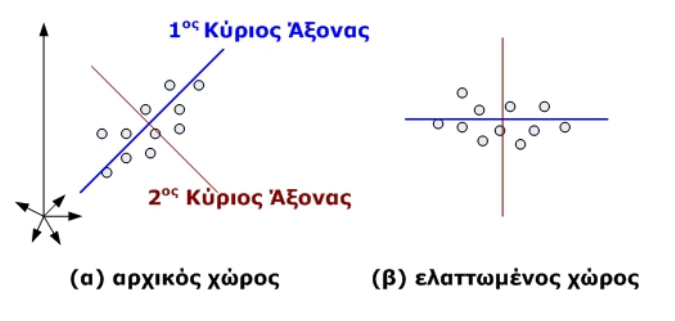
\includegraphics[width=\textwidth,height=20cm,keepaspectratio]{pictures/5.2pca.png} 
\caption{Παράδειγμα λειτουργίας της μεθόδου \en{PCA}}\label{figure5.2}
\end{figure}

\subsection{Η τεχνική \en{SMOTE}}

Για την αντιμετώπιση του προβλήματος της ανισορροπίας των δεδομένων (\en{imbalanced data}), οι ερευνητές Μηχανικής Μάθησης χρησιμοποιούν:
\begin{enumerate}
    \item Είτε τεχνικές \en{oversampling}, οι οποίες έχουν ως στόχο να δημιουργήσουν στιγμιότυπα σε κλάσεις που θεωρούνται μειονότητες σε σχέση με το μέσο όρο
    \item Είτε τεχνικές \en{undersampling} που ακολουθούν την αντίστροφη διαδικασία, αφαιρούν δηλαδή στιγμιότυπα απο τις κλάσεις με το μεγαλύτερο πληθυσμό.
\end{enumerate}

Οι δύο αυτές διαδικασίες χρήζουν ιδιαίτερης προσοχής ώστε, στην πρώτη περίπτωση να μη δημιουργηθούν χαμηλής ποιότητας και αξίας δεδομένα, ή αλλιώς θόρυβος, και στη δεύτερη περίπτωση, να μη χαθεί χρήσιμη πληροφορία. 

Ο αλγόριθμος του \en{SMOTE (Synthetic Minority Oversampling Technique)}, όπως υποδηλώνει και το πλήρες όνομα του, εντοπίζει την κλάση ή τις κλάσεις με τα ελλιπή στιγμιότυπα και συνθέτει νέα στιγμιότυπα από τα ήδη υπάρχοντα, με σκοπό την εξισορρόπηση των στιγμιότυπων μεταξύ των κλάσεων του συνόλου δεδομένων. Τα στιγμιότυπα αυτά είναι συνθετικά και δημιουργούνται αξιοποιώντας τις τιμές των ήδη υπαρχόντων στιγμιοτύπων. 
Εφαρμόζει την προσέγγιση KNN \en{(k-nearest neighbours)}, με βάση τους K πλησιέστερους γείτονες, δημιουργεί τα συνθετικά δείγματα στον χώρο της μειοψηφίας. Ο αλγόριθμος παίρνει τα διανύσματα χαρακτηριστικών από τους πλησιέστερους γείτονές του και υπολογίζει την απόσταση μεταξύ αυτών των διανυσμάτων. Η διαφορά πολλαπλασιάζεται με τυχαίο αριθμό μεταξύ (0, 1) και προστίθεται στο χαρακτηριστικό.

Στο σχήμα ~\ref{figure5.9} γίνεται μια προσπάθεια επεξήγησης του τρόπου λειτουργίας του αλγορίθμου της τεχνικής \en{SMOTE} γραφικά. Τα στιγμιότυπα των κλάσεων με το μεγαλύτερο πληθυσμό απεικονίζονται με μπλε χρώμα, τα στιγμιότυπα των κλάσεων που αποτελούν μειονότητες απεικονίζονται με πράσινο χρώμα και τα συνθετικά στιγμιότυπα που δημιουργεί η τεχνική \en{SMOTE} απεικονίζονται με κόκκινο χρώμα και ενσωματώνονται στην κλάση-μειονότητα:

\begin{figure} [ht!]
\centering
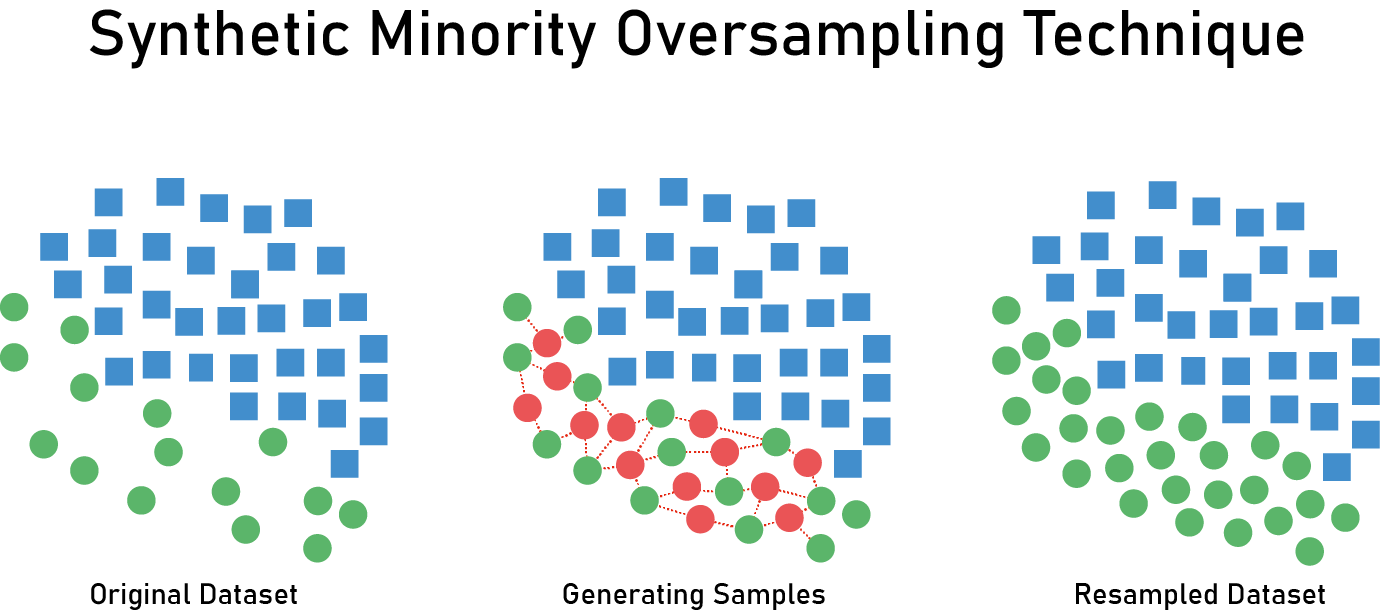
\includegraphics[width=\textwidth,height=12cm,keepaspectratio]{pictures/smote example.png} 
\caption{Γραφική επεξήγηση της λειτουργίας του αλγορίθμου \en{SMOTE}}\label{figure5.9}
\end{figure}


\section{Αλγόριθμοι Ταξινόμησης (\en{Classification Algorithms})}

\subsection{Λογιστική Παλινδρόμηση (\en{Logistic Regression})}
Η Λογιστική Παλινδρόμηση (\en{Logistic Regression}), ή εναλλακτικά το λογιστικό υπόδειγμα πιθανότητας, αποτελεί στην ουσία ένα μη γραμμικό μοντέλο ταξινόμησης των τιμών μιας μεταβλητής απόκρισης Υ με βάση τη θεωρία πιθανοτήτων. Στο λογιστικό μοντέλο το σφάλμα δεν ακολουθεί την κανονική κατανομή. Επίσης, η εξαρτημένη μεταβλητή Υ είναι δυική \en{(boolean)}, δηλαδή παίρνει τιμές 0 και 1 και αναφέρεται στην πραγματοποίηση ή όχι ενός γεγονότος. Η λογιστική παλινδρόμηση χρσηιμοποιείται εκτενώς σε πολλές εφαρμογές όπου επιδιώκεται η πραγματοποίηση πρόβλεψης της παρουσίας ή απουσίας κάποιου χαρακτηριστικού ή γενονότος.
Πρακτικά, αναπτύσσεται μια μη γραμμική συνάρτηση, βάσει της οποίας υπολογίζεται η πιθανότητα ένα στοιχείο να έχει ή όχι το χαρακτηριστικό το οποίο εξετάζεται την κάθε στιγμή. 

Η συνάρτηση αυτή ονομάζεται λογιστική συνάρτηση και εκφράζεται από τον τύπο:

\begin{figure} [ht!]
\centering
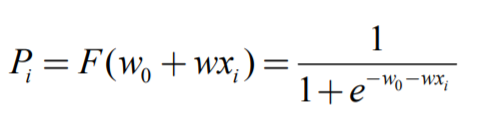
\includegraphics[width=\textwidth,height=2cm,keepaspectratio]{pictures/2logisticR.png} \label{figure2.0}
\end{figure}
\clearpage

Τέλος, αξίζει να σημειωθεί ότι πρώτος ο \en{James A. Ohlson}, το 1980, χρησιμοποίησε το λογιστικό υπόδειγμα πιθανότητας σε έρευνα του σχετικά με την πρόβλεψη της πτώχευσης επιχειρήσεων. \cite{ohlson1980}



%%%%%%%%%%%%%%%%%%   NAIVE BAYES   %%%%%%%%%%%%%%%%%% 

\subsection{\en{Naïve Bayes}}
Ο αλγόριθμος \en{Naïve Bayes} αποτελεί ένα σύνολο πιθανολογικών μοντέλων μηχανικής μάθησης, με σκοπό την επίλυση προβλημάτων ταξινόμησης, το οποίο βασίζεται στο θεώρημα πιθανοτήτων \en{Bayes}.
Αξιοποιώντας το Θεώρημα \en{Bayes} ο αλγόριθμος, για κάθε δεδομένο εισόδου (πχ μήνυμα κειμένου, \en{tweet}, τίτλος άρθρου), προβλέπει, μέσα απο ένα σύνολο δεδομένων διακριτών κατηγοριών, την κατηγορία στην οποία ανήκει. Η πρόβλεψη αποτελεσμάτων από μη επισημασμένα δεδομένα έχει ως προϋπόθεση την ανεξαρτησία μεταξύ των χαρακτηριστικών (\en{features}), μια προϋπόθεση που εάν στην πραγματικότητα αποτελούσε εφικτό στόχο θα απλοποιούσε σημαντικά τη διαδικασία μάθησης.


Ο αλγόριθμος \en{Naïve Bayes} χαρακτηρίζεται ως πιθανολογικός λόγω του ότι η πρόβλεψη γίνεται αποδίδοντας μια πιθανότητα για κάθε δεδομένη κατηγορία και επιστρέφοντας εκείνη με τη μεγαλύτερη πιθανότητα. Οι πιθανότητες υπολογίζονται μεσω του θεωρήματος \en{Bayes}, το οποίο αξιολογεί πιθανολογικά το κάθε χαρακτηριστικό (\en{feature}) ξεχωριστά βάσει της ήδη υπάρχουσας γνώσης που σχετίζεται με αυτό.

\subsubsection{Θεώρημα \en{Bayes}}

\begin{align*}
    P(A/B) = \frac{P(A) * P(B/A)}{P(B)}
\end{align*}
όπου Α και Β γεγονότα.
\begin{itemize}
    \item \en{P(A)} και \en{P(B)} είναι οι πιθανότητες των A και B που είναι ανεξάρτητα μεταξύ τους.
    \item \en{P(A/B),} η υπό συνθήκη πιθανότητα, είναι η πιθανότητα του A δεδομένου του B να είναι αληθής.
    \item \en{P(B/A),} είναι η πιθανότητα του B δεδομένου του A να είναι αληθής.
\end{itemize} \cite{bayesTheorem}
% https://en.wikipedia.org/wiki/Bayes%27_theorem   CITE

To Θεώρημα \en{Bayes} συσχετίζει την τρέχουσα πιθανότητα με την αρχική πιθανότητα. Μπορεί δηλαδή να υπολογιστεί η πιθανότητα να συμβεί ένα γεγονός Α δεδομένου ενός γεγονότος Β. Όταν πρόκειται για πρόβλημα ταξινόμησης το γεγονός Β αναφέρεται στην απόδειξη και το γεγονός Α στην υπόθεση.


\begin{align*}
    P(class/features) = \frac{P(class) * P(features/class)}{P(features)}
\end{align*}

\begin{itemize}
    \item \en{P(class/features)} : εκ των υστέρων πιθανότητα
    \item \en{P(class)} : εκ των προτέρων πιθανότητα κλάσης
    \item \en{P(features/class)} : Δεσμευμένη Πιθανότητα
    \item \en{P(features)} : εκ των υστέρων πιθανότητα ταξινομητή
\end{itemize}


Η \en{P(class/features)} καλείται συνάρτηση πιθανοφάνειας της κλάσης σε σχέση με το χαρακτηριστικό και χρησιμοποιείται για 
να δηλώσει ότι η κατηγορία για την οποία η συνάρτηση έχει μεγάλη τιμή έχει μεγαλύτερη πιθανότητα να  είναι η  σωστή κατηγορία αναφορικά με την πρόβλεψη. Να σημειωθεί ότι το γινόμενο της  πιθανοφάνειας και της εκ των προτέρων πιθανότητας είναι αυτό που  καθορίζει την τιμή της εκ των υστέρων πιθανότητας.

Η βιβλιοθήκη \en{Scikit-learn} της \en{Python} προσφέρει τρεις τύπους μοντέλων  \en{Naïve Bayes}:
\begin{enumerate}
    \item \en{Multinomial Naïve Bayes}: Το συγκεκριμένο μοντέλο χρησιμοποιείται κατα κόρον σε προβλήματα που αφορούν την ταξινόμηση κειμένου σε κατηγορίες που το χαρακτηρίζουν.
    \item \en{Bernoulli Naïve Bayes:} Η διαφοροποίηση του με το \en{Multinomial Naïve Bayes} έγκειται στο οτι οι τιμές πρόβλεψης είναι αυστηρά δυαδικές\en{(boolean)}. Αυτό σημαίνει οτι για κάθε δεδομένο η απάντηση του αλγορίθμου είναι της μορφής ΝΑΙ/ΟΧΙ, κάνοντας το μοντέλο χρήσιμο σε αντίστοιχες εφαρμογές όπως, για παράδειγμα, στην αξιολόγηση ενός κειμένου ως υβριστικού ή όχι.
    \item \en{Gaussian Naïve Bayes:} Στα \en{gaussian} μοντέλα, όπως υποδηλώνει και το όνομα, οι προβλέψεις για κάθε κλάση ακολουθούν την κατανομή \en{Gauss} (Σχήμα ~\ref{figure2.1}). Επομένως οι προβλέψεις εκφράζονται με συνεχείς και όχι διακριτές τιμές. 
\end{enumerate}

\begin{figure}\centering
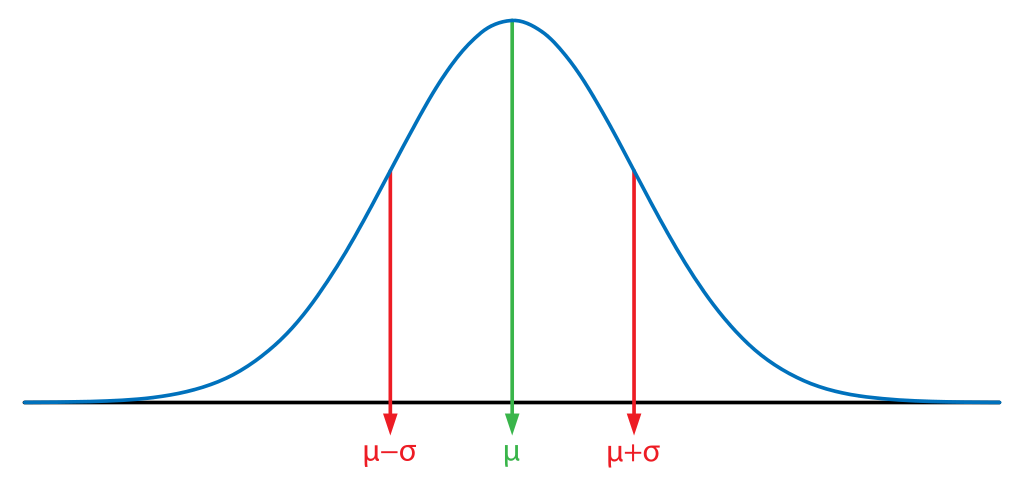
\includegraphics[width=\textwidth,height=14cm,keepaspectratio]{pictures/2.1Gaussian_distribution.png} \caption{Η κατανομή \en{Gauss} (Κανονική κατανομή)}\label{figure2.1}
\end{figure}

\begin{frame}{}
        \hspace{0.5cm} Η συνάρτηση πυκνότητας πιθανότητας της κανονικής κατανομής είναι:
        \begin{equation}
        f(x | \mu,\,\sigma^{2})=\frac{1}{\sqrt{2\,\pi \sigma^{2}}}\,\E^{-\frac{\left(x-\mu\right)^2}{2\,\sigma^2} }
        \end{equation}
        Όπου
        \begin{itemize}
            \item '${\mu}$' είναι η μέση τιμή της μεταβλητής
            \item '${\sigma}$' είναι η τυπική απόκλιση
            \item '${\sigma^2}$' είναι η διακύμανση. 
        \end{itemize}
\end{frame}

%%%%%%%%%%%%%%%%%%   SVM   %%%%%%%%%%%%%%%%%% 

\subsection{\en{Supported Vector Machine}}

Το πρωταρχικό μοντέλο του αλγορίθμου \en{SVM (Supported Vector Machine)} δημιουργήθηκε από τους \en{Vladimir Vapnik} και \en{Alexey Chervonenkis} το 1963. Το 1992, προτάθηκε από τoυς \en{Bernhard Boser, Isabelle Guyon} και \en{Vladimir Vapnik} ένα πιο ισχυρό μοντέλο το οποίο χρησιμοποιείται για την ταξινόμηση δεδομένων σε κατηγορίες και αποτελεί μια τεχνική που χρησιμοποιείται ευρέως στην κατηγοριοποίηση κειμένου λόγω της μεγάλης αποδοτικότητας της. Ο λόγος που θεωρείται ένας απ τους καλύτερους κατηγοριοποιητές στην ταξινόμηση κειμένου είναι η ικανότητα του μοντέλου να διαχειρίζεται μεγάλα σύνολα χαρακτήρων, όπως είναι ένα κείμενο φυσικής γλώσσας.

Ο αλγόριθμος λειτουργεί ως εξής:

Αρχικά παίρνει ως είσοδο το σύνολο δεδομένων εκπαίδευσης (\en{training set}) και δημιουργεί μία απεικόνιση του σε ένα πολυδιάστατο διανυσματικό χώρο. Σε αυτόν το χώρο προσπαθεί να εντοπίσει ένα πεδίο το οποίο να διαχωρίζει τα δύο υποσύνολα δεδομένων, ανάλογα με το αν ανήκουν ή όχι στην εκάστοτε κατηγορία, μεγιστοποιώντας την απόσταση ανάμεσα στο πεδίο και στα δεδομένα εκατέρωθεν του, όπως φαίνεται στο Σχήμα ~\ref{figure2.2}, όπου το διαχωριστικό πεδίο απεικονίζεται με πράσινο χρώμα και ο διαχωρισμός των δύο υποσυνόλων είναι ευδριάκριτος.

Χρησιμοποιώντας έπειτα αυτό το πεδίο, το οποίο ονομάζεται \en{hyperplane.}, ο αλγόριθμος είναι ικανός να προβλέψει αποτελεσματικά την κατηγορία στην οποία ανήκει ένα άγνωστο μέχρι στιγμής δεδομένο εισόδου χαρτογραφώντας το στο χώρο και αποφασίζει σε ποια μεριά του διαχωριστικού πεδίου ανήκει. 

Ο τρόπος του αλγορίθμου να επιλέξει ένα από τα πολλά διαχωριστικά πεδία που θα μπορούσαν να δημιουργηθούν στο διανυσματικό χώρο είναι να επιλέξει το πεδίο με τη μεγαλύτερη απόσταση από τα δεδομένα του εκπαιδευτικού συνόλου, μειώνοντας έτσι τις πιθανότητες σφάλματος στην πρόβλεψη.
\begin{figure}[h!]
\centering
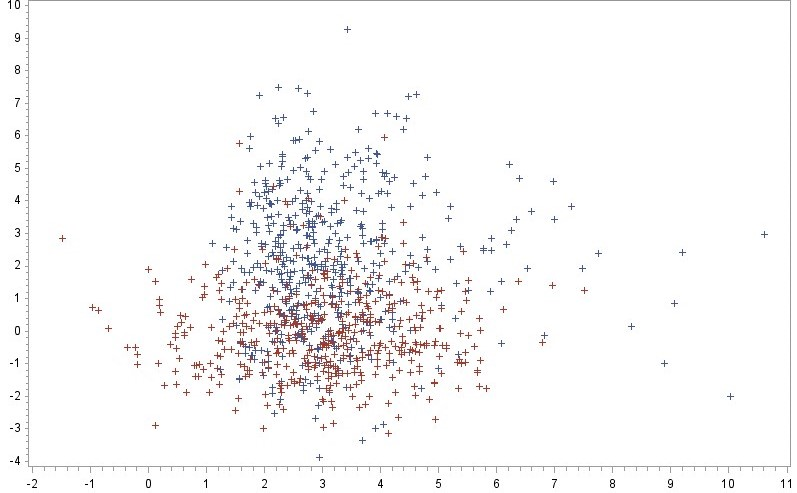
\includegraphics[width=\textwidth,height=10cm,keepaspectratio]{pictures/2.2svmScatter.jpg}
\caption{\en{Scatter Plot:} Παράδειγμα χαρτογράφησης δεδομένων σε χώρο δύο διαστάσεων}
\label{figure2.2}
\end{figure}

\begin{figure}[h!]
\centering
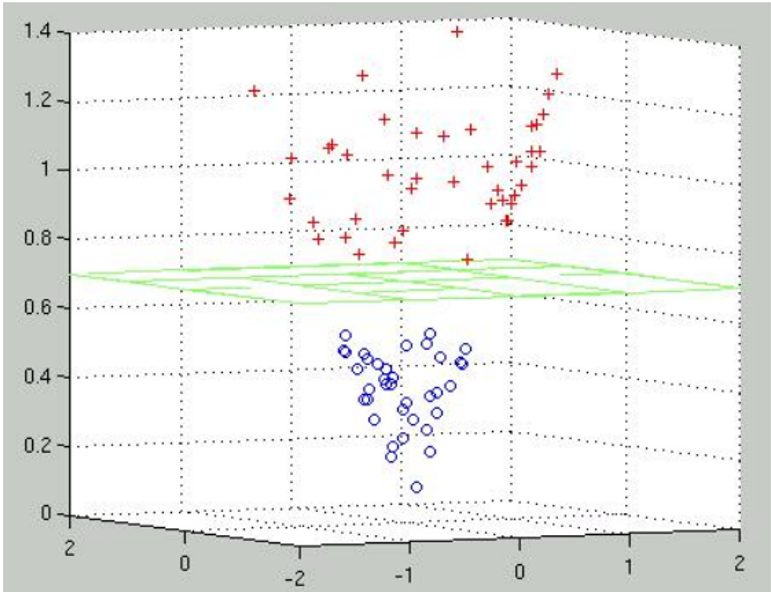
\includegraphics[width=\textwidth,height=10cm,keepaspectratio]{pictures/2.3svm.png}
\caption{Αλγόριθμος \en{SVM:} Παράδειγμα χαρτογράφησης δεδομένων στον πολυδιάστατο διανυσματικό χώρο}
\label{figure2.3}
\end{figure}


\en{\subsection{\en{k Nearest Neighbors - kNN}}

\clearpage
\section{Νευρωνικά Δίκτυα \en{(Neural Networks - NN)}}

Ομοίως με τον άνθρωπο, ένα νευρωνικό δίκτυο απαιτεί εκπαίδευση για να λειτουργήσει σωστά. Η εκπαίδευση περιλαμβάνει τον προσδιορισμό των κατάλληλων συντελεστών βαρών μεταξύ των συνάψεων του, η οποία επιτυγχάνεται μέσω αλγορίθμων που βοηθούν στην εκμάθηση του περιβάλλοντος και τη βελτίωση της απόδοσης του. Η εκπαίδευση ενός νευρωνικού δικτύου είναι μια σταδιακή διαδικασία, η οποία ακολουθεί καθορισμένους κανόνες. Επαναλαμβανόμενες διαδικασίες ρύθμισης των βαρών στις συνάψεις μεταξύ των επιπέδων επιτρέπουν στο νευρωνικό δίκτυο να αποκτήσει περισσότερη "γνώση". Με αυτόν τον τρόπο, το νευρωνικό δίκτυο μπορεί να διπλασιάσει τον όγκο των γνώσεων του, καθιστώντας το πιο αποτελεσματικό στο να ανταποκρίνεται στις απαιτήσεις του περιβάλλοντος στο οποίο επιδρά.





\subsection{\en{Βαθιά Μάθηση (Deep Learning)}}
Η τεχνολογία του deep learning είναι μια προηγμένη μέθοδος μηχανικής μάθησης, η οποία βασίζεται στη χρήση νευρωνικών δικτύων, μια κατηγορία αλγορίθμων με μακρά ιστορία που ξεκινά από τον αλγόριθμο Perceptron του Rosenblatt το 1957 \cite{deep1}  και φτάνει στις σύγχρονες τεχνικές. Στον τομέα της οπτικής αναγνώρισης, οι Geoffrey Hinton και Yann LeCun έχουν κάνει σημαντικές προσπάθειες στην εξέλιξη αυτής της τεχνολογίας.

Αυτά τα δίκτυα είναι σχεδιασμένα να αναλύουν και να εξάγουν χρήσιμες πληροφορίες από μεγάλα σύνολα δεδομένων, σε αντίθεση με τις παραδοσιακές μεθόδους που βασίζονται σε κανόνες και χειροκίνητη επεξεργασία δεδομένων.
Μαθηματικά, τα νευρωνικά δίκτυα είναι μη γραμμικές συναρτήσεις που εκτελούν πολλαπλά επίπεδα επεξεργασίας για την εξαγωγή συμπερασμάτων από τα δεδομένα εισόδου. Η μέθοδος αυτή επιτρέπει στα νευρωνικά δίκτυα να εξάγουν χαρακτηριστικά χωρίς τη χρήση ανθρώπινης παρέμβασης στην επεξεργασία των δεδομένων. Μέσω της επιβλεπόμενης μάθησης, τα νευρωνικά δίκτυα μπορούν να αναγνωρίσουν πρότυπα και σχέσεις στα δεδομένα εισόδου. 

Για παράδειγμα, μπορούν να ταξινομήσουν εικόνες σε διαφορετικές κατηγορίες χρησιμοποιώντας ετικέτες. Σε αυτό το παράδειγμα, η μηχανική μάθηση μπορεί να χρησιμοποιηθεί για να εκπαιδεύσει ένα μοντέλο να αναγνωρίζει εάν μια εικόνα περιέχει ζώο ή άνθρωπο, βασιζόμενο σε ένα σύνολο εκπαίδευσης που περιλαμβάνει εικόνες ταξινομημένες ως απεικόνιση ανθρώπου ή απεικόνιση ζώου. Ενώ για τον ανθρώπινο εγκέφαλο φαντάζει εύκολο να διαχωριστεί η εικόνα ενός ανθρώπου από εκείνη ενός άλλου ζώου, είναι αρκετά δύσκολο να προσδιορίσει κανείς εν είδει μιας ακολουθίας βημάτων (αυτό που στην επιστήμη της πληροφορικής ονομάζεται αλγόριθμος) την διαδικασία που ακολουθεί η λογική σκέψη του για να κάνει αυτήν την ταξινόμηση. 

Το μοντέλο μηχανικής μάθησης μπορεί να εξάγει αυτόματα χαρακτηριστικά από τις εικόνες, όπως γωνίες και συνήθως χρησιμοποιείται ένα νευρωνικό δίκτυο για να εκπαιδευτεί σε αυτά τα χαρακτηριστικά. Στη συνέχεια, το μοντέλο μπορεί να χρησιμοποιηθεί για να ταξινομήσει νέες εικόνες, βασιζόμενο στις παραμέτρους με τις οποίες έχει εκπαιδευτεί.

Η μηχανική μάθηση λοιπόν, χρησιμοποιείται για να δώσει σε έναν υπολογιστή την ικανότητα να αναγνωρίζει πρότυπα και να προβλέπει αποτελέσματα με βάση τα δεδομένα που έχει "δει". Στην ουσία, ο υπολογιστής εκπαιδεύεται με ένα σύνολο δεδομένων εισόδου-εξόδου και μαθαίνει να αναγνωρίζει συσχετίσεις μεταξύ αυτών των δεδομένων, ώστε να μπορεί να κάνει προβλέψεις για νέα δεδομένα.

Το επιθυμητό αποτέλεσμα της επιβλεπόμενης μάθησης επιτυγχάνεται μέσω της βελτιστοποίησης και παραμετροποίησης μιας πολυπαραγοντικής ευέλικτης συνάρτησης, η οποία θα πρέπει να αφομοιώνει και να αναγνωρίζει τις ετικέτες μιας σειράς
ετικετοποιημένων δεδομένων (labelled dataset), γνωστή ως σετ δεδομένων εκπαίδευσης (training dataset). Ο αλγόριθμος αναζητά μέσα στο χώρο όλων των πιθανών τιμών των παραμέτρων με στόχο να προσδιορίσει τη βέλτιστη συνάρτηση η οποία θα ταιριάζει με τα ετικετοποιημένα παραδείγματα με τη μεγαλύτερη δυνατή ακρίβεια. Στη συνέχεια θα χρησιμοποιήσει τη συνάρτηση αυτή για να ταξινομήσει νέες άγνωστες εικόνες που θα δοθούν προς ταξινόμηση.

Ουσιαστικά, τα νευρωνικά δίκτυα είναι τόσο ευέλικτα που μπορούν να προσεγγίσουν μαθηματικά οποιαδήποτε συνάρτηση, χρησιμοποιώντας ένα μεγάλο αριθμό απλών συναρτήσεων που συνδέονται με διάφορους τρόπους. Μπορούν να συνδεθούν σειριακά ή παράλληλα, με τη μία μετασχηματιστική λειτουργία να αποτελεί την είσοδο για την επόμενη ή με πολλές μετασχηματιστικές λειτουργίες να εφαρμόζονται παράλληλα στα δεδομένα και το αποτέλεσμα να συνδυάζεται. Μια από τις βασικές τεχνικές της μηχανικής μάθησης είναι η υπερβολική προσαρμογή (overfitting), όπου το μοντέλο εκπαιδεύεται να ανταποκρίνεται πολύ στα δεδομένα εκπαίδευσης και δεν μπορεί να γενικεύσει σε νέα δεδομένα. Για να αποφευχθεί αυτό, χρησιμοποιούνται τεχνικές όπως η απόσυρση (dropout) και η κανονικοποίηση (regularization).

Αν και ιστορικά η Βαθιά Μάθηση ξεκινά να υπάρχει με την εμφάνιση του αλγόριθμου \en{«perceptron»}, σήμερα χρησιμοποιείται ευρέως ως σύχγρονη τεχνική σε διάφορες εφαρμογές. Η Βαθιά Μάθηση είναι το πεδίο της Μηχανικής Μάθησης που χρησιμοποιεί πιο σύνθετες μορφές μοντέλων, διαχωρισμένων σε πολλά ιεραρχικά επίπεδα. Πιο συγκεκριμένα, αυτά τα μοντέλα ονομάζονται «Βαθιά νευρωνικά δίκτυα», ξεκινούν από ένα επίπεδο δεδομένων εισόδου, το οποίο στη συνέχεια περνά ξεχωριστά από αρκετά «κρυφά» επίπεδα αλλοιώντας κάθε φορά τα χαρακτηριστικά των δεδομένων εισόδου. Με αυτόν τον τρόπο, το μοντέλο αναπτύσσεται ως προς την κατανόηση των δεδομένων εισόδου, με αποτέλεσμα τη σταδιακή βελτίωση του αλγόριθμου ως προς νέα διαθέσιμα δεδομένα. 

Ουσιαστικά, η υπολογιστική μηχανή αποκτά τη δυνατότητα να λειτουργεί με παρόμοιο τρόπο, όπως ο ανθρώπινος εγκέφαλος, να πράττει, δηλαδή, μαθαίντας φυσικά μέσα από παραδείγματα. Με τους αλγόριθμους της Βαθιάς Μάθησης, οι συνδέσεις των δεδομένων γίνονται με τη μορφή «δένδρου» σε πολλαπλά ιεραχικά επίπεδα, γεγονός που θυμίζει τις νευρωνικές συνδέσεις του ανθρώπινου εγκεφάλου, ο οποίος επίσης χρησιμοποιεί απλές υπολογιστικές μονάδες, γνωστές ως νευρώνες, για να πραγματοποιεί πολύπλοκους υπολογισμούς. Ωστόσο, είναι σημαντικό να σημειωθεί ότι τα νευρωνικά δίκτυα δεν αποτελούν ακριβή αντιγραφή του ανθρώπινου εγκεφάλου και οι σύγχρονες επιλογές αρχιτεκτονικών και συναρτήσεων έχουν σχεδιαστεί χωρίς να περιορίζονται στο να αντικατοπτρίζουν πλήρως τον τρόπο λειτουργίας του. \cite{3.5}, \cite{3.9}

\clearpage
\subsection{\en{Μοντέλο Νευρωνικού Δικτύου (Neural Network Model)}}
Ένα νευρωνικό δίκτυο αποτελείται από πολλά μικρά υποσυστήματα που ονομάζονται νευρώνες. Κάθε νευρώνας λαμβάνει είσοδο από άλλους νευρώνες ή από το περιβάλλον και παράγει μια έξοδο, η οποία μπορεί να χρησιμοποιηθεί ως είσοδος σε άλλους νευρώνες.

\begin{figure}[h!]
\centering
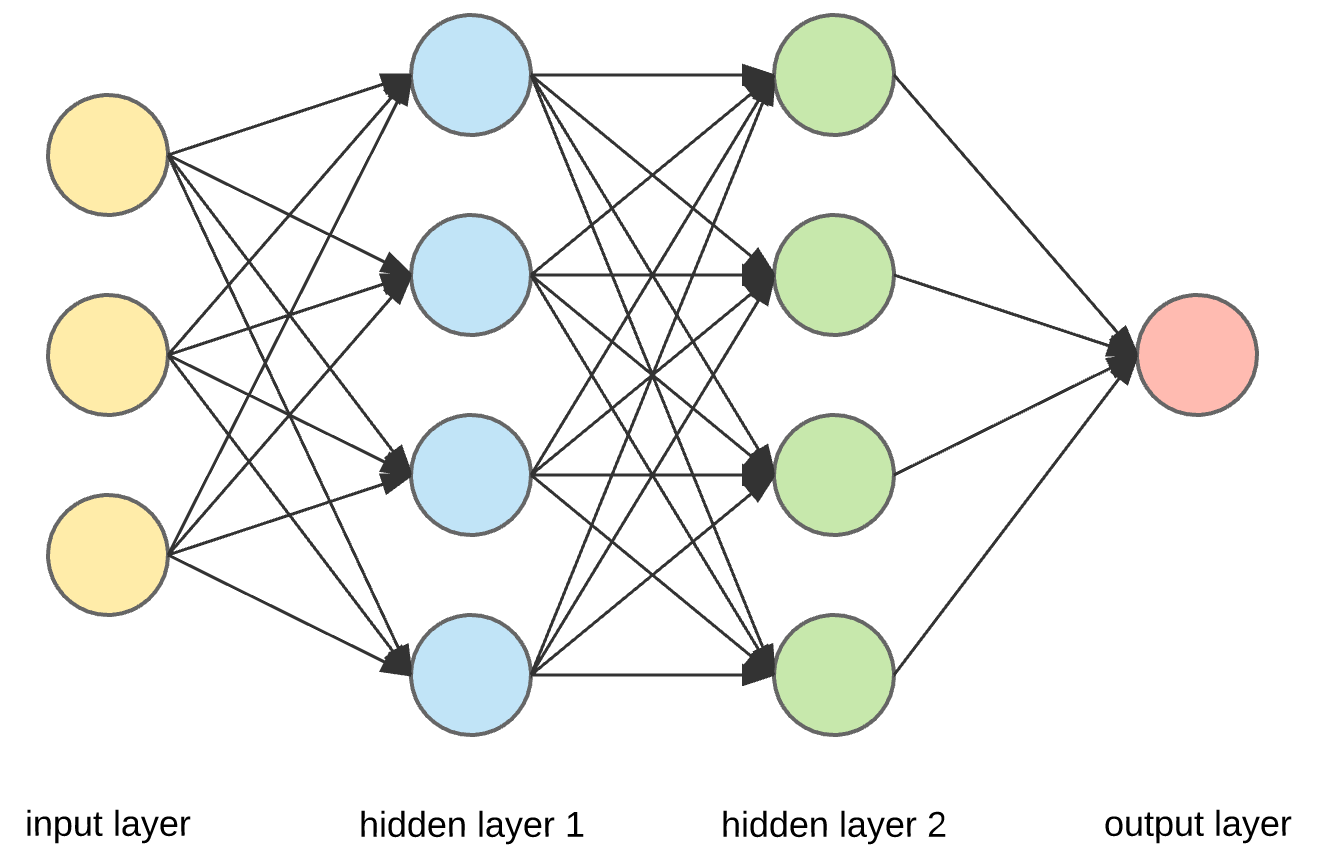
\includegraphics[width=\textwidth,height=10cm,keepaspectratio]{pictures/neural_network.png}
\caption{Απλό μοντέλο νευρωνικού δικτύου που αποτελείται επίπεδα εισόδου, επίπεδα εξόδου και κρυφά επίπεδα.}
\label{figure2.4}
\end{figure}

Κάθε νευρώνας έχει ένα σύνολο βαρών που αντιστοιχεί στις εισόδους του, καθώς και μια συνάρτηση ενεργοποίησης, η οποία καθορίζει το επίπεδο εξόδου που θα παραχθεί, δεδομένων των εισόδων και των σχετικών βαρών.

Τα νευρωνικά δίκτυα είναι οργανωμένα σε επίπεδα (layers), όπου κάθε στρώμα αποτελείται από πολλούς νευρώνες που επεξεργάζονται την ίδια είσοδο. Τα επίπεδα στα νευρωνικά δίκτυα συνήθως χωρίζονται σε τρία είδη: επίπεδο εισόδου (input layer), κρυφό επίπεδο (hidden layer) και επίπεδο εξόδου (output layer).

Το επίπεδο εξόδου αποτελείται από μια ή περισσότερες μονάδες που παράγουν την τελική έξοδο του δικτύου, δηλαδή την πρόβλεψη ή την ταξινόμηση του δεδομένου εισόδου.

Η διαδικασία εκπαίδευσης του νευρωνικού δικτύου συνήθως περιλαμβάνει τη ρύθμιση των βαρών των συνδέσμων μεταξύ των νευρώνων, ώστε να ελαχιστοποιηθεί η απόκλιση της έξοδου του δικτύου από την επιθυμητή έξοδο. Η διαδικασία αυτή γίνεται μέσω της χρήσης ενός αλγορίθμου βελτιστοποίησης, όπως η μέθοδος των ελαχίστων τετραγώνων ή η μέθοδος της ανάδρασης προς τα πίσω (backpropagation).

}

